\chapter{Experiments: Lattices}
\label{ch:regular-tilings}

% (TODO): Overall: standard deviations.

% (TODO): Remember to always specify specifics of experiment setups for all
% experiments

% (TODO): t!
\begin{figure*}[t]
  \centering
  \begin{subfigure}{.32\textwidth}
    \centering
    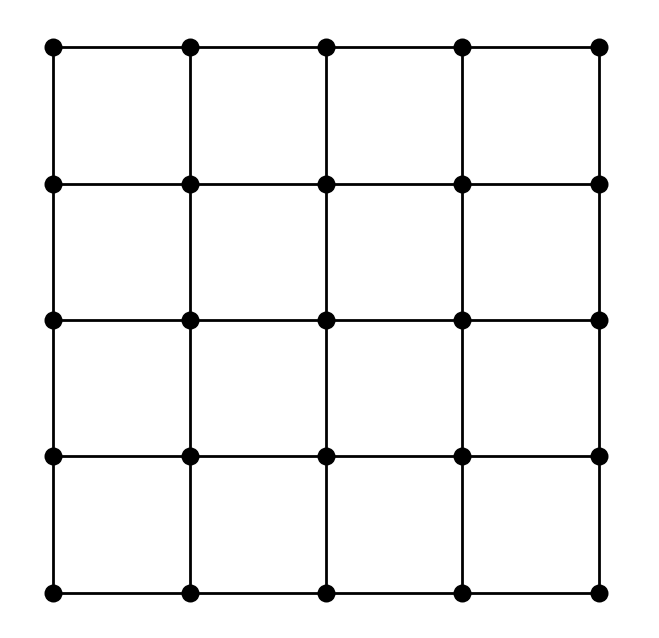
\includegraphics[width=1.0\linewidth]{figures/square.png}
    \label{fig:rt-square}
  \end{subfigure}
  \begin{subfigure}{.32\textwidth}
    \centering
    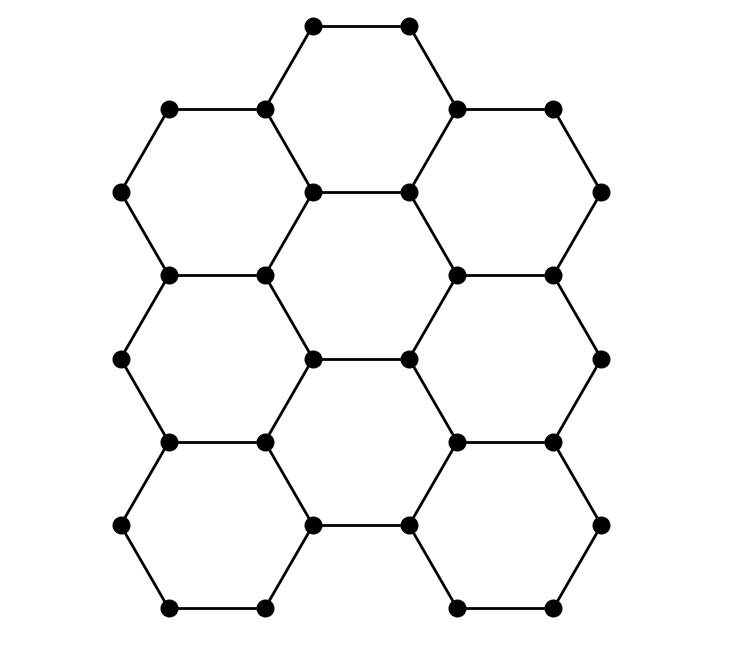
\includegraphics[width=1.0\linewidth]{figures/hex.png}
    \label{fig:rt-hex}
  \end{subfigure}
  \begin{subfigure}{.32\textwidth}
    \centering
    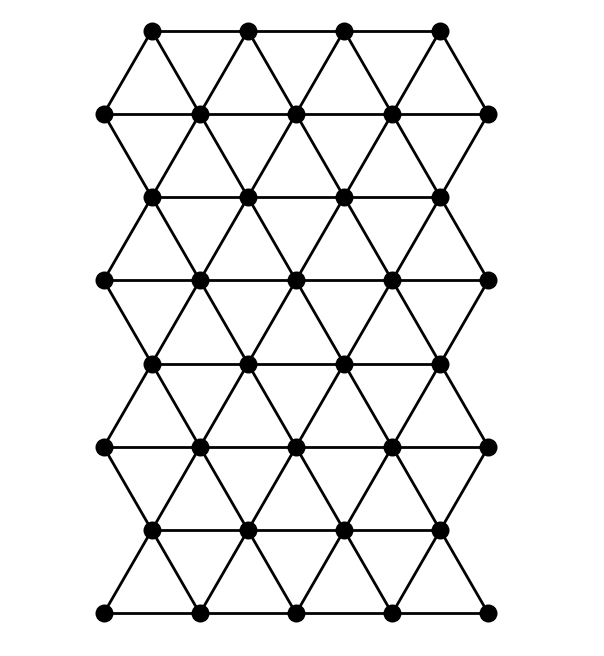
\includegraphics[width=1.0\linewidth]{figures/triangular.png}
    \label{fig:rt-tri}
  \end{subfigure}
  \caption{
    Types of lattices investigated for their quality as reservoir
topologies. Investigated tilings include square (a), hexagonal (b), and
triangular (c).
  }
  \label{fig:regular-tilings}
\end{figure*}

Lattice models are common in computational physics
\cite{lavis_equilibrium_2015}. Understanding important models of computational
physics in reservoir contexts is thus crucial to advance physical RC
methodology. For example, the Ising model with dipole moments of atomic spins
\cite{jensen_computation_2018}, spin-torque oscillator arrays
\cite{tsunegi_physical_2019}, and the Ginzburg-Landau equation
\cite{opala_neuromorphic_2019}, describe systems that are employed on a
two-dimensional lattice, and have been used in reservoir settings. In this
chapter, we therefore investigate lattice networks as more realistic models of
physical reservoirs.

We explore the properties that lattice graphs exhibit as reservoirs by
structuring internal nodes in this manner. Lattice graphs may be embedded in
Euclidean space to form regular tilings, of which there three in two-dimensional
space: square, hexagonal and triangular, which are all depicted in Figure
\ref{fig:regular-tilings}. Other, more complicated tiling schemes
exist. Semiregular, often called uniform, tilings are created using two or more
faces. However, complicated grids are left outside the scope of this thesis, as
our primary focus is the fundamental applicability of lattice layouts, not
comparing the performance between them.

Reservoirs are created by replacing the reservoirs of ESN models with the
adjacency matrix generated for lattice models. For each experiment,
$\mathbf{W}^{res}$ is then scaled to a spectral radius of 0.9, as this is
equivalent to scaling the coupling, or spacing, between nodes in a physical
system. Beyond this, our reservoir model remains the same as that of the ESN.

\textcolor{red}{
  Perhaps a paragraph summarizing each section.
}

\section{Reservoir Quality of Lattices}

\subsection{Synopsis}

First, we evaluate the default quality of lattice reservoirs with the NARMA-10
benchmark. Reservoirs are generated by embedding internal nodes in a metric
space, much like in Figure \ref{fig:regular-tilings}, and connecting neighboring
pairs with an edge of unit length. Nodes along the edges are not connected to
the opposite side of the lattice, making the lattice aperiodic. Lastly, unit
weight of all edges are scaled by the appropriate scalar to allow a spectral
radius of 0.9.

\subsection{Results and Discussion}

% (TODO): t!
\begin{figure}[t]
  \centering
  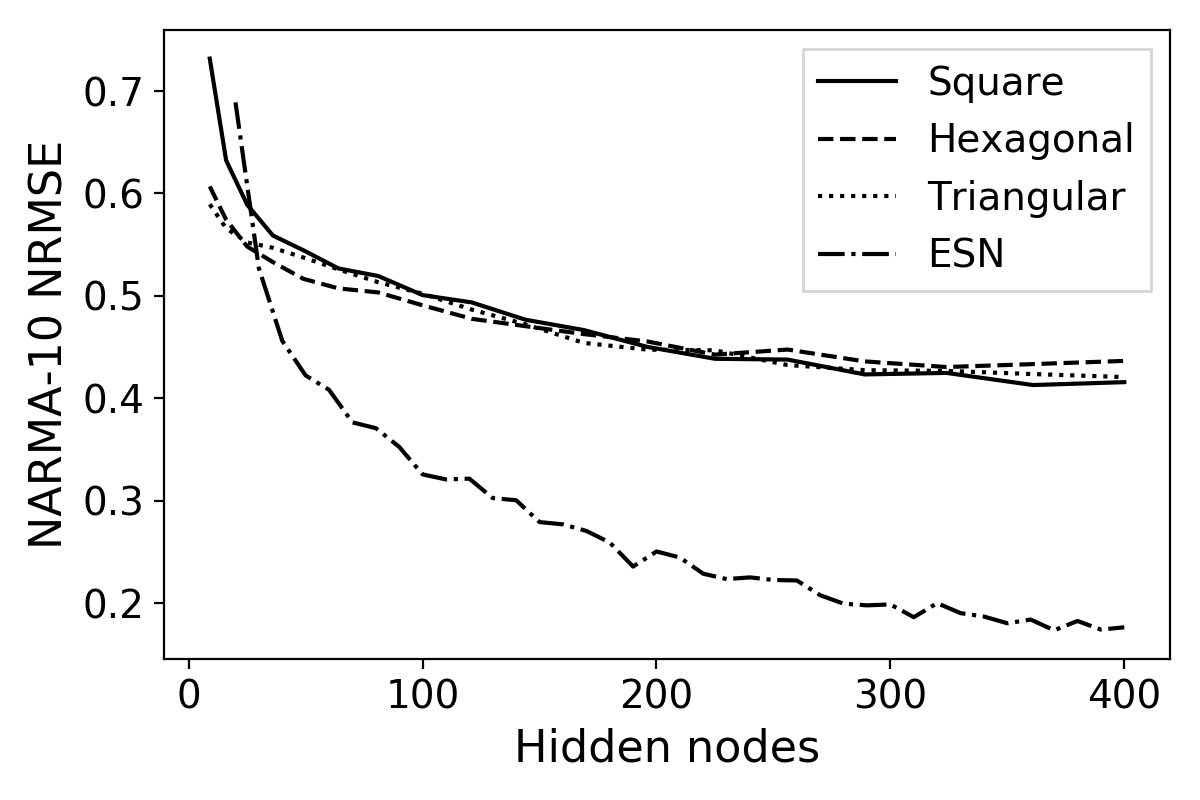
\includegraphics[width=3.5in]{figures/regular-tilings-performance.png}
  \caption{
    NARMA-10 NRMSE of square, hexagonal, and triangular regular tilings as
reservoir topologies.
  }
  \label{fig:rt-performance}
\end{figure}

Figure \ref{fig:rt-performance} shows how reservoir error scales with reservoir
size. We see that restricting reservoir topologies to lattice structures results
in a significant performance penalty. Additionally, little difference is seen
between the three types of tilings.

% (TODO): t!
\begin{figure*}[t]
  \centering
  \begin{subfigure}{.32\textwidth}
    \centering
    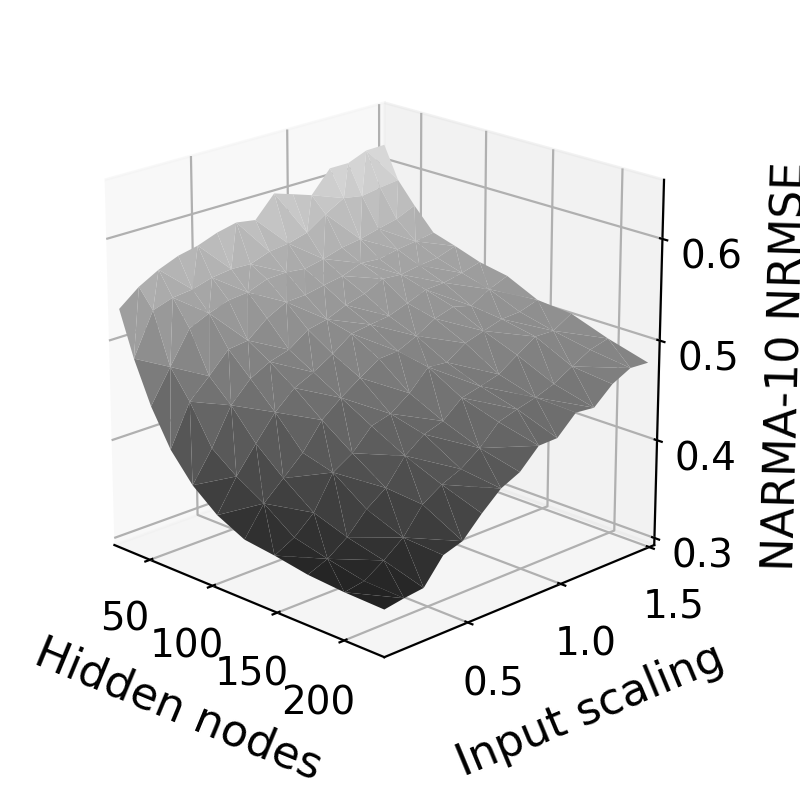
\includegraphics[width=1.0\linewidth]{figures/regular-tilings-performance-is-sq.png}
    \caption{}
    \label{fig:rt-is-square}
  \end{subfigure}
  \begin{subfigure}{.32\textwidth}
    \centering
    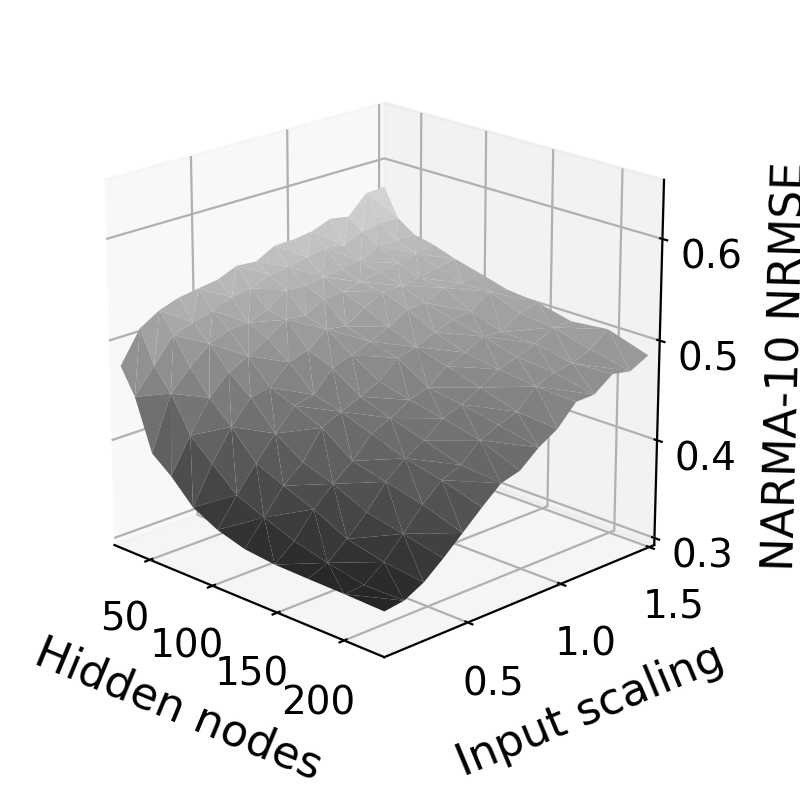
\includegraphics[width=1.0\linewidth]{figures/regular-tilings-performance-is-hex.png}
    \caption{}
    \label{fig:rt-is-hex}
  \end{subfigure}
  \begin{subfigure}{.32\textwidth}
    \centering
    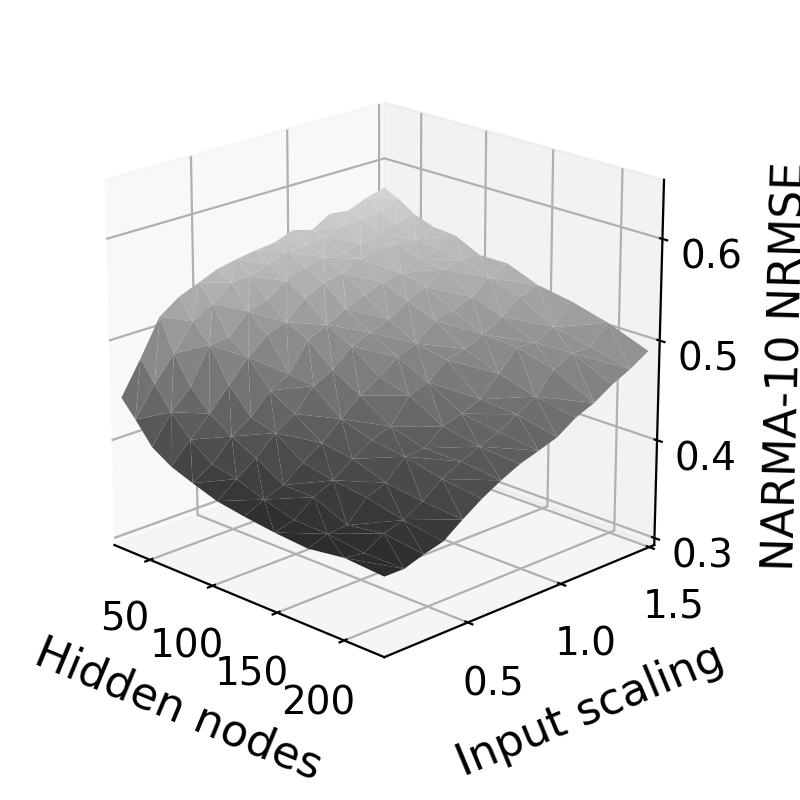
\includegraphics[width=1.0\linewidth]{figures/regular-tilings-performance-is-tri.png}
    \caption{}
    \label{fi:rt-is-tri}
  \end{subfigure}
  \caption{
    Regular tilings investigated for their quality as reservoir topologies, here
as a function of reservoir size and input scaling. Investigated topologies
include square (a), hexagonal (b), and triangular (c) regular tilings.
  }
  \label{fig:rt-performance-is}
\end{figure*}

In Section \ref{sec:dist-func}, it was discovered that reservoirs modeling
random geometric graphs exhibited low memory retention. The symptoms are similar
here: the lattice reservoirs perform worse than a delay line would, and only
perform marginally better with an increasing size. Figure
\ref{fig:rt-performance-is} illustrates the effect of scaling the magnitude of
the input. Again, we see clearly see reservoirs favoring low input scaling
values.

We interpret these results to indicate that the structure imposed by an
undirected lattice shifts the point of criticality described in
\ref{sec:criticality}. When input scaling is lessened such that the required
memory capacity for the benchmark task is reached, the error diminishes rapidly,
and the existing reservoir dynamics work as intended.

Curiously, the NRMSE differs only slightly between the three types of
lattice. It seems that it is the overall lattice structure that is important,
not the specific type of tiling implementing it. We therefore argue that the
different tilings, which in practice dictate the amount of incident edges per
vertex, work mostly as minor tuning parameters. The idea that overall structure
is important is in accordance with our findings in \ref{sec:restore}, concluding
that \textit{how information flows} in the network is vital.

Input scaling decreased the benchmark error of lattice reservoirs, but the best
performing networks of Figure \ref{fig:rt-performance-is} are not quite
comparable to the ESN. For example, square grid reservoirs of size 200 benchmark
a mean NRMSE of around 0.35, while corresponding ESNs average around 0.25.

Overall, it is interesting that undirected lattice reservoirs perform as well as
they do. On the other hand, the distribution of the input weights are drawn from
a uniform distribution in the interval [-0.5, 0.5], letting internal nodes see
varying representations of the input signal. As physical substrates may differ
in the input schemes they offer, the input scheme will be further investigated
in the next section.

To summarize, we have in this section found undirected lattice reservoirs to
provide promising results. A key discovery of Chapter \ref{ch:rgg} is the
importance of a directed flow of information, and whether directedness also
improves lattice models is the topic of the next section.

\section{Lattices with Directed Edges}

\subsection{Synopsis}

% (TODO): ref.
\textcolor{red}{
Using knowledge obtained in Chapter ?, we modify the resulting networks to have
directed edges, and scale the input magnitude to find a suitable one.
}

\subsection{Results and Discussion}

% (TODO): t!
\begin{figure*}[t]
  \centering
  \begin{subfigure}{.40\textwidth}
    \centering
    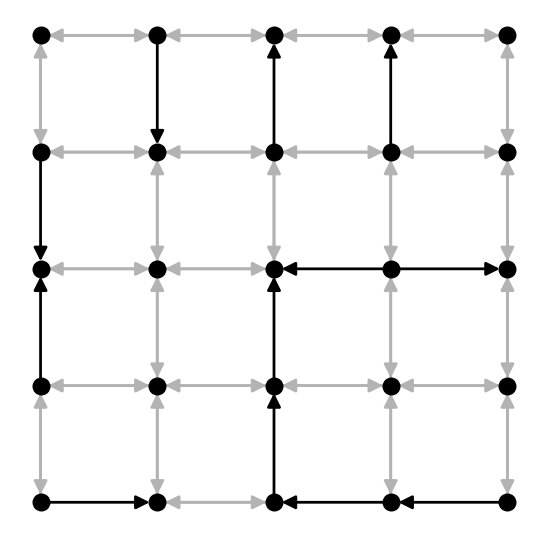
\includegraphics[width=1.0\linewidth]{figures/dir_lattice_025.png}
    \caption{}
    \label{fig:dir-lattice-a}
  \end{subfigure}
  \hspace{25pt}
  \begin{subfigure}{.40\textwidth}
    \centering
    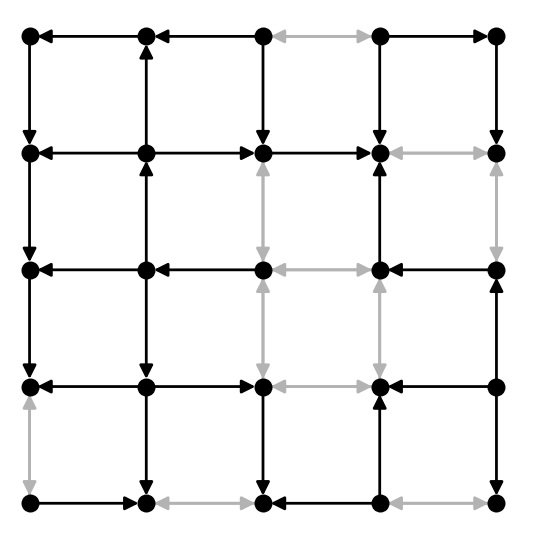
\includegraphics[width=1.0\linewidth]{figures/dir_lattice_075.png}
    \caption{}
    \label{fig:dir-lattice-b}
  \end{subfigure}
  \caption{
    Example square grids where 25\% (a) and 75\% (b) of the undirected edges are
made directed instead.
  }
  \label{fig:dir-lattice}
\end{figure*}

% (TODO): t!
\begin{figure*}[t]
  \centering
  \begin{subfigure}{.32\textwidth}
    \centering
    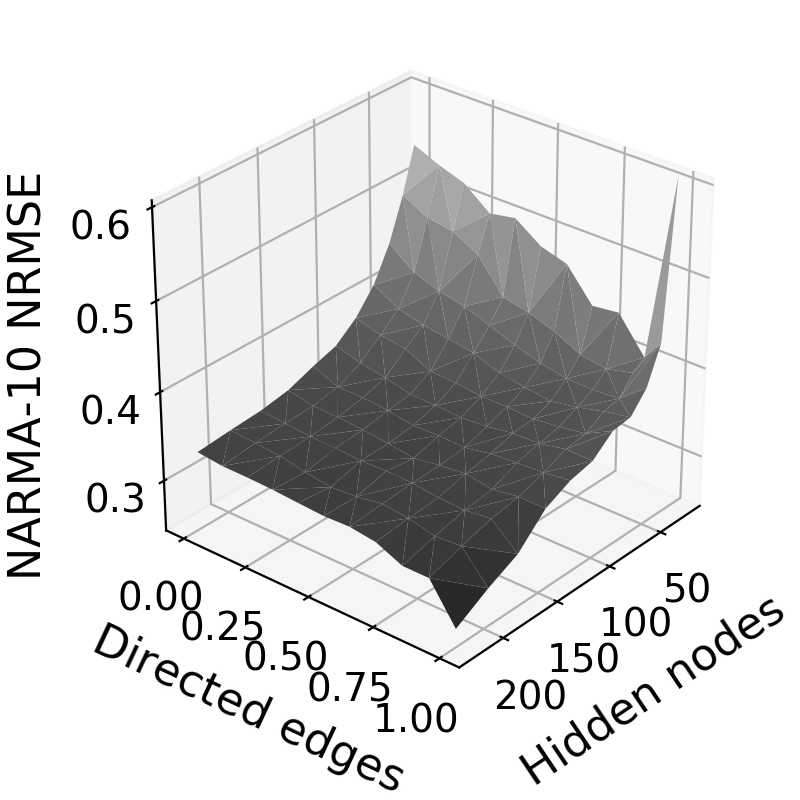
\includegraphics[width=1.0\linewidth]{figures/rt-dir-perf-sq.png}
    \caption{}
    \label{fig:rt-dir-perf-trisurf-sq}
  \end{subfigure}
  \begin{subfigure}{.32\textwidth}
    \centering
    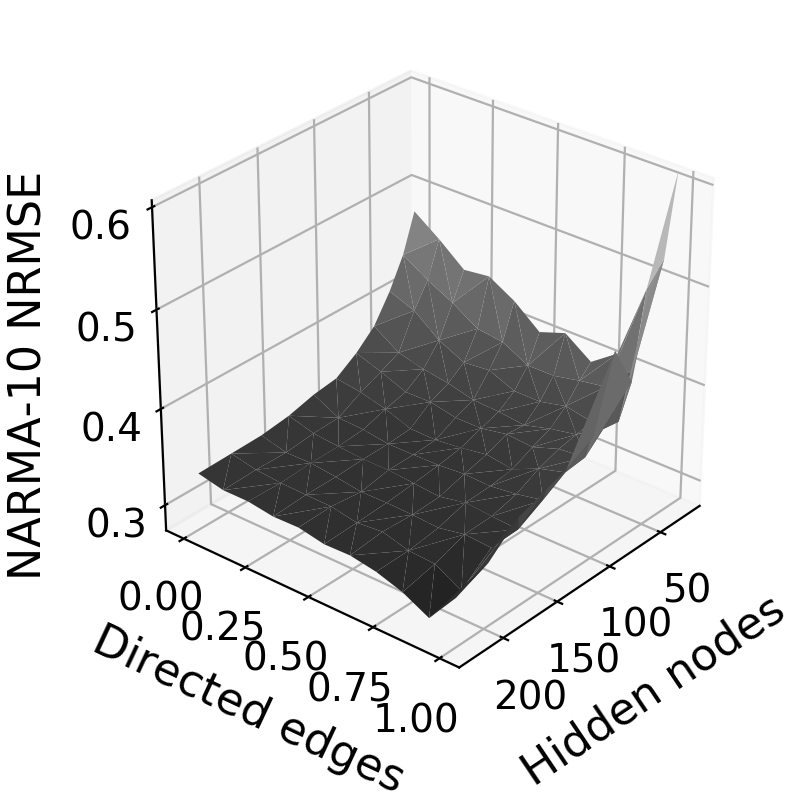
\includegraphics[width=1.0\linewidth]{figures/rt-dir-perf-hex.png}
    \caption{}
    \label{fig:rt-dir-perf-trisurf-hex}
  \end{subfigure}
  \begin{subfigure}{.32\textwidth}
    \centering
    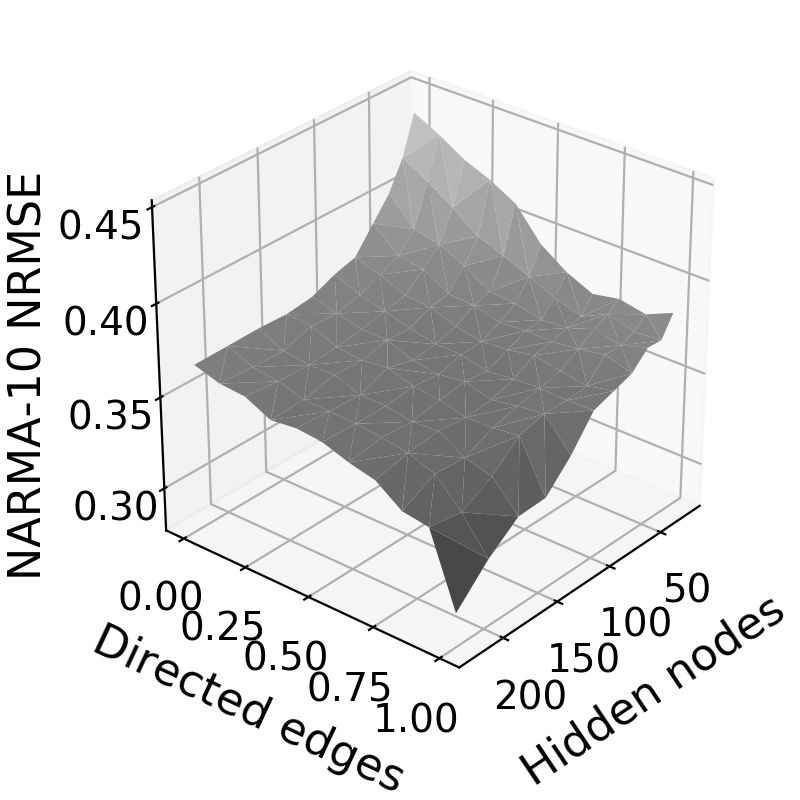
\includegraphics[width=1.0\linewidth]{figures/rt-dir-perf-tri.png}
    \caption{}
    \label{fig:rt-dir-perf-trisurf-tri}
  \end{subfigure}
  \caption{
    \textcolor{red}{No caption yet.}
  }
  \label{fig:rt-dir-perf-trisurf}

  \centering
  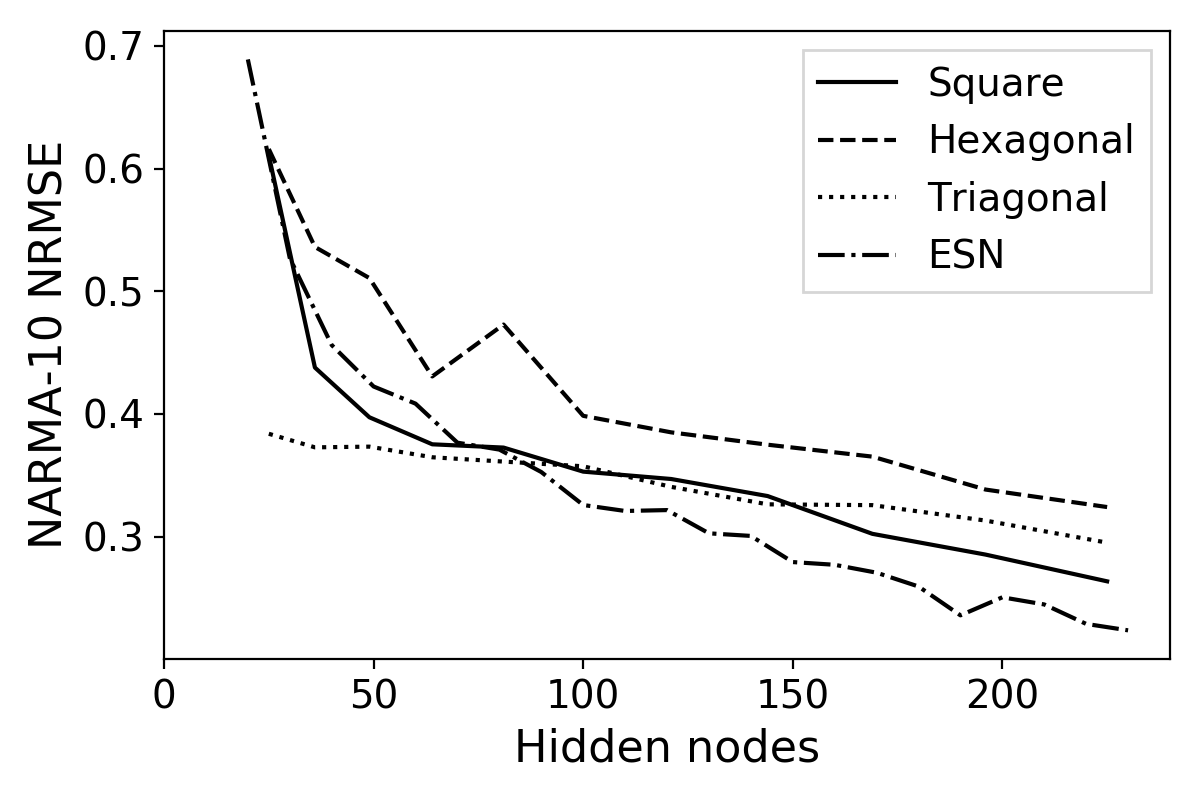
\includegraphics[width=3.5in]{figures/rt-dir-perf.png}
  \caption{\textcolor{red}{No caption yet here.}}
  \label{fig:rt-dir-perf}
\end{figure*}

\textcolor{red}{
  We see that directed edges make the grids perform quite close to ESNs on the
NARMA-10 dataset. We choose the square lattice to move further, as they are all
quite similar, but the square one seems most stable and performs very well.
}

\begin{figure}
  \centering
  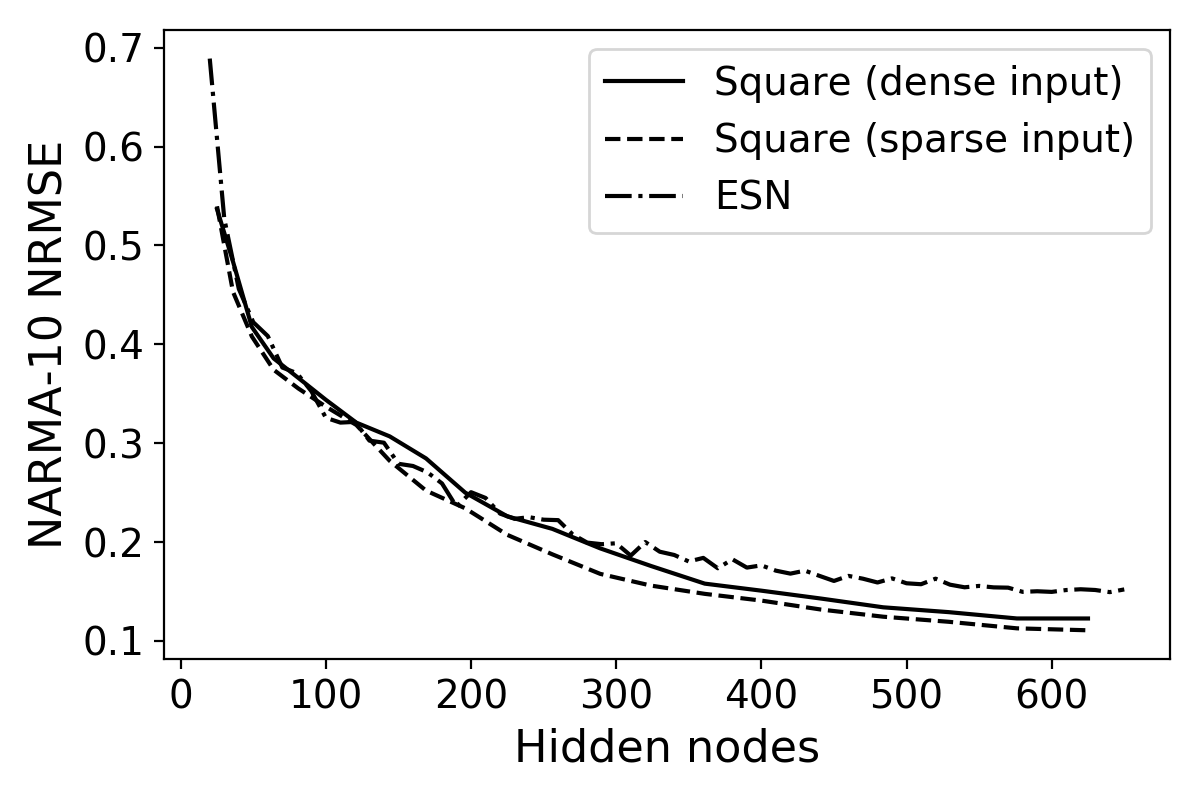
\includegraphics[width=3.5in]{figures/rt-performance-big.png}
  \caption{\textcolor{red}{No caption here yet.}}
  \label{fig:rt-performance-big}
\end{figure}

\textcolor{red}{
  When we introduce a global input scheme, the square grids get even
better. This is crazy. The square grids do not plateau nearly as much as the
ESNs. In fact they get much better. We also add sparse input matrices, which
means only 50\% of the hidden nodes see the input.
}

% (TODO): t!
\begin{table}[t]
  \centering
  \begin{center}
    \caption{
      \textcolor{red}{
        Simple weighting scheme of square grids. Displayed values are given as
an average across 10 experiment runs (std. dev.). Reservoir connectivity density
in ESNs is 10\%.
      }
    }
    \label{tab:sq-global-input}
    \begin{tabular}{c c c c c}
      \hline
      \thead{Reservoir type} & \thead{Hidden \\ nodes} & \thead{Unique \\ input weights} & \thead{Unique \\ reservoir weights} & \thead{NARMA-10 \\ NRMSE} \\
      \hline
      \rule{0pt}{2.5ex}Square grid & 100 & 1 & 1 & 0.346 (0.019) \\
      Square grid & 225 & 1 & 1 & 0.245 (0.022) \\
      Square grid & 400 & 1 & 1 & 0.168 (0.009) \\
      \rule{0pt}{3ex}ESN & 100 & 100 & 997 (26) & 0.388 (0.019) \\
      ESN & 225 & 225 & 5098 (74) & 0.282 (0.019) \\
      ESN & 400 & 400 & 16070 (113) & 0.215 (0.021)\rule[-1ex]{0pt}{0pt} \\
      \hline
    \end{tabular}
  \end{center}
\end{table}

\textcolor{red}{
  Performance wise? Input is actually just adding a single scalar. The internal
matrix is very sparse. Compared to ESN this should be pretty nice. We can do a
pretty short benchmark, just raw, unfair comparison.
}

\textcolor{red}{
  Key difference to CRJ: there is only one input weight, not a distribution with
signedness.
}

% (TODO): t!
\begin{figure*}[t]
  \centering
  \begin{subfigure}{.49\textwidth}
    \centering
    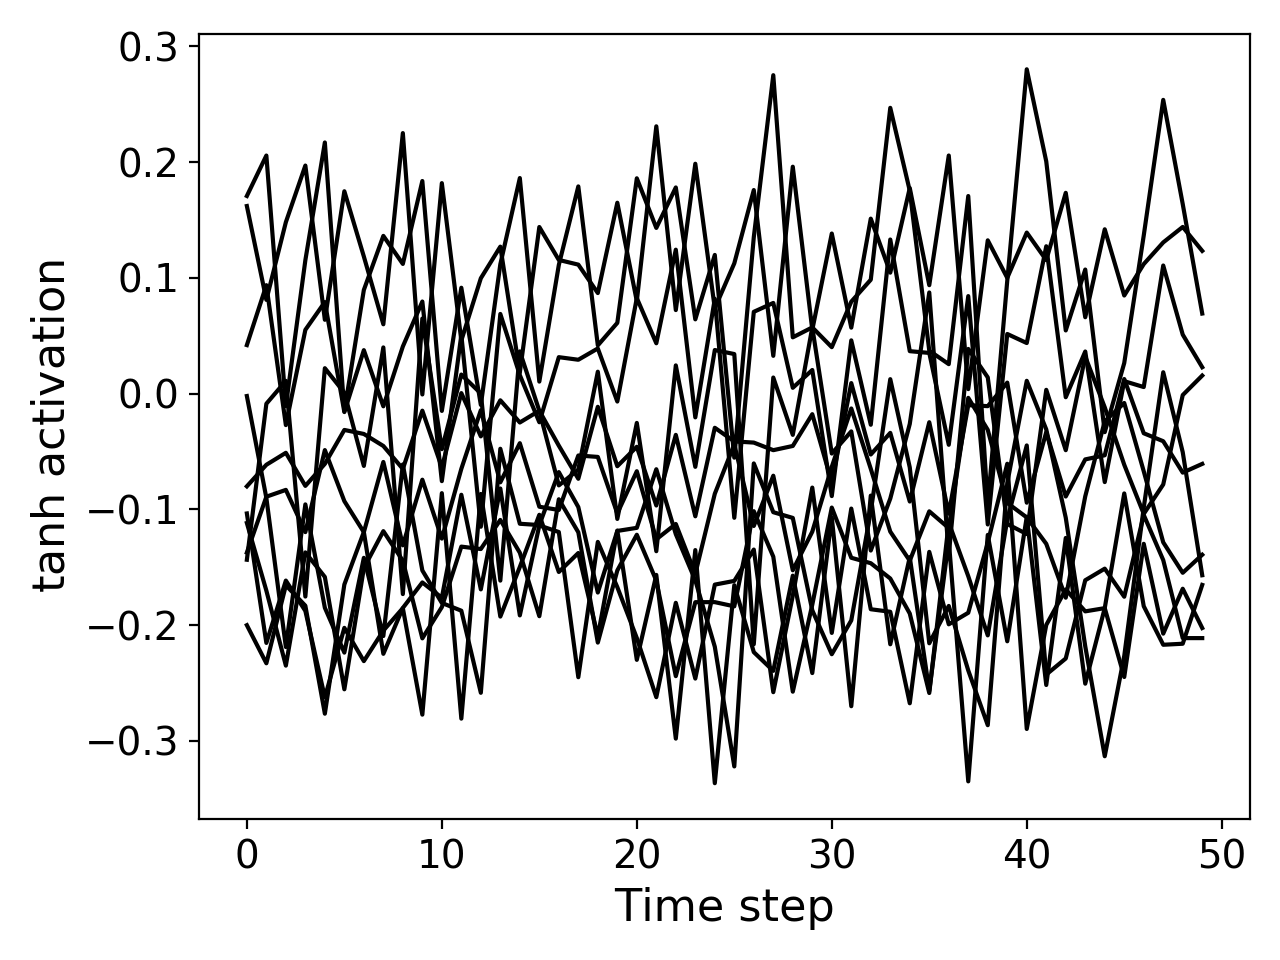
\includegraphics[width=1.0\linewidth]{figures/esn-activations.png}
    \caption{}
    \label{fig:activations-a}
  \end{subfigure}
  \begin{subfigure}{.49\textwidth}
    \centering
    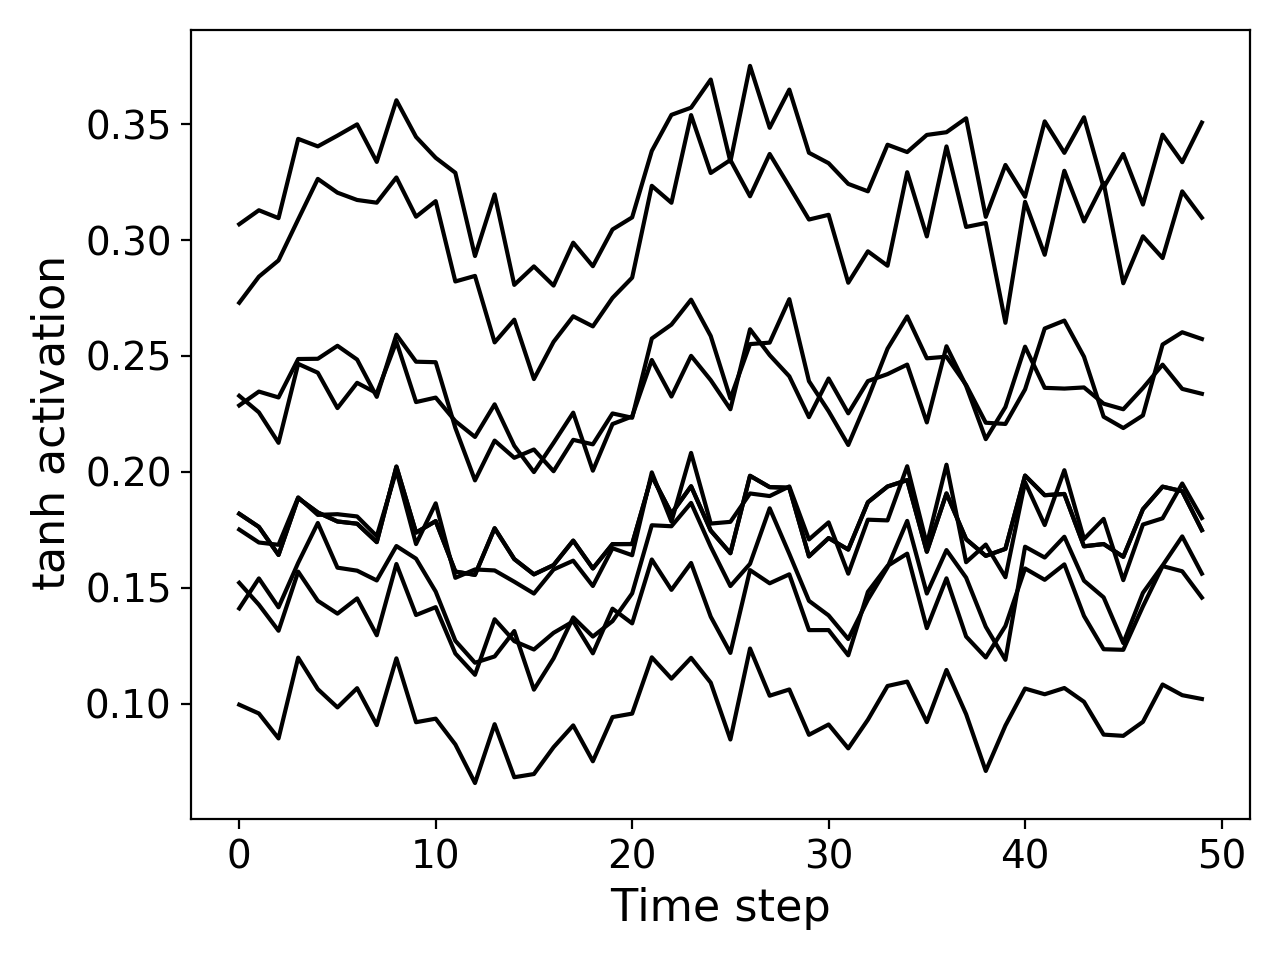
\includegraphics[width=1.0\linewidth]{figures/sq-activations.png}
    \caption{}
    \label{fig:activations-b}
  \end{subfigure}
  \caption{
    \textcolor{red}{
      This is only 10 of the nodes to give an example without cluttering too
much. Square grid has only positive activations, and the input is clearly
visible, while the ESN is sporadic, random.
    }
  }
  \label{fig:activations}
\end{figure*}

\textcolor{red}{
  After looking at the activations here, all positive, one may consider other
sigmoid functions of course, but experiments showed $tanh$ to work just fine.
}

\textcolor{red}{
  We should maybe also compare MC and KQ/G to that of ESNs, as independent
metrics. We see that the square grids have a much lower kernel quality,
i.e. less dynamics, which may impact performance. However, some studies with
Mackey-Glass indicate that it will also work for that. So there is this
trade-off to make the square grid work, in that the dynamics are lessened for
memory, but it \textit{works}, which is the key. Also, very important to look
back to the discrepancy between Rodan and Dale here, as there we see something
completely similar with rings. Good conclusion to draw!
}

\textcolor{red}{
  Should we include experiments with harder NARMA? I think there is already
quite a lot of information, so this might not really be necessary.
}

\textcolor{blue}{
  ``The experimental results clearly demonstrate that our very simple deter-
ministic reservoir constructions have the potential to significantly outper-
form standard ESN randomized reservoirs. We propose that instead of relying on
unnecessary stochastic elements in reservoir construction, one can obtain
superior (and sometimes superior by a large margin) perfor- mance by employing
the simple regular unidirectional circular topology with bidirectional jumps
with fixed cycle and jump weights. However, it is still not clear exactly what
aspects of dynamic representations in the reservoirs are of importance and
why.'' From cycle reservoirs with jumps paper. The part about stochastic
elements is quite interesting.
}

\section{Nonlinear Dynamics in Square Grids}

\subsection{Synopsis}

\textcolor{red}{
  I think maybe a section on KQ+G, and then Mackey-Glass 17 in addition could be
good. MG17 should be re-tuned input scaling and spectral radius since its a new
task, obviously. We can compare KQ with that of Dale et al. structure, and reach
a similar conclusion to that of the background, with the discrepancy between
ring and crj.
}

\subsection{Results and Discussion}

% (TODO): t!
\begin{figure*}[t]
  \centering
  \begin{subfigure}{.49\textwidth}
    \centering
    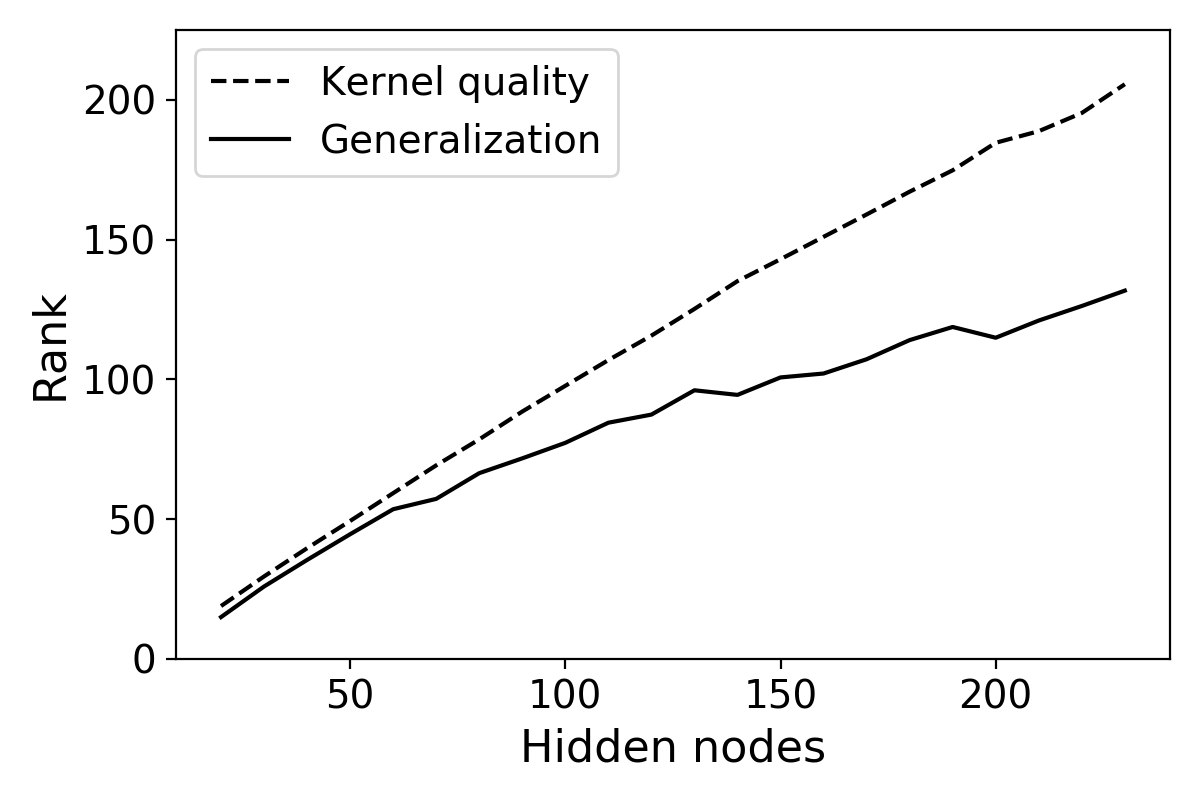
\includegraphics[width=1.0\linewidth]{figures/esn-rank.png}
    \caption{}
    \label{fig:rank-a}
  \end{subfigure}
  \begin{subfigure}{.49\textwidth}
    \centering
    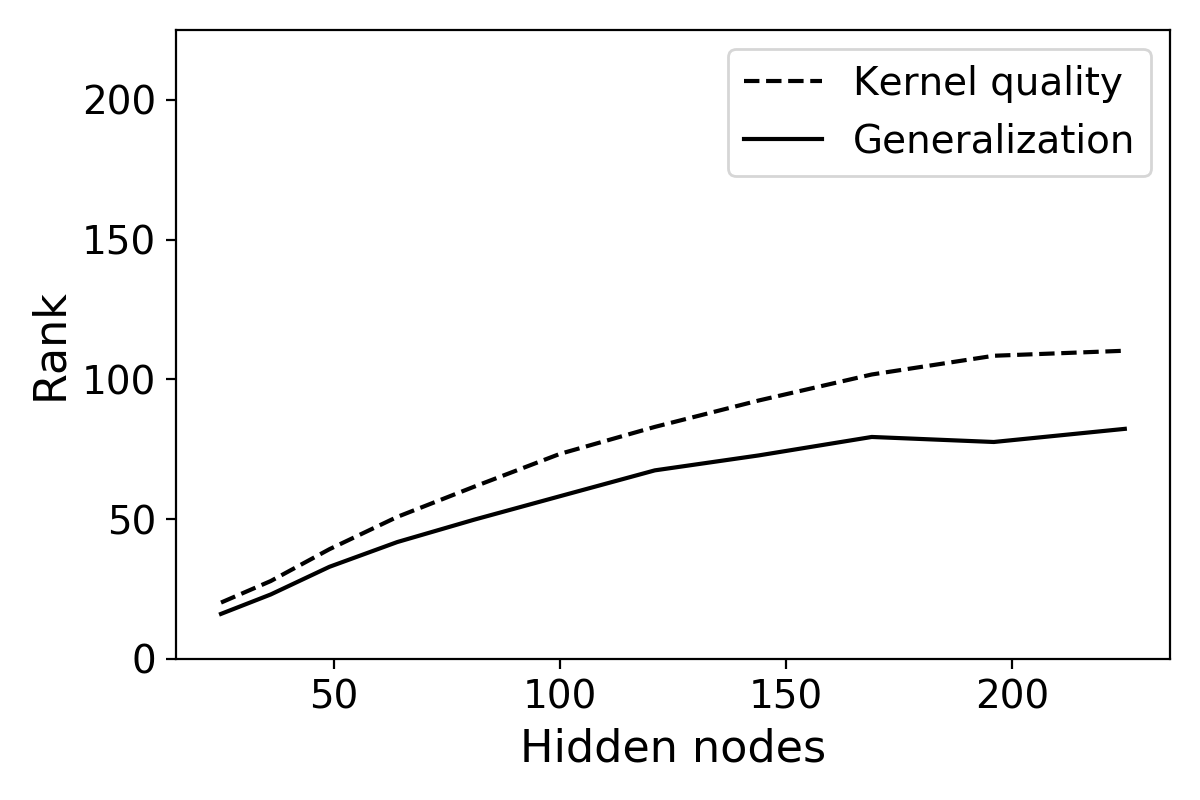
\includegraphics[width=1.0\linewidth]{figures/sq-rank.png}
    \caption{}
    \label{fig:rank-b}
  \end{subfigure}
  \caption{
    \textcolor{red}{
      No caption yet.
    }
  }
  \label{fig:rank}
\end{figure*}

\textcolor{red}{
  The ESN can reach most of the behavior space, as described in Dale et al. We
tune the spectral radius to 0.7, achieving very results to before, but a bit
more interesting KQ/G space. Easier to compare with lattices.
}

% (TODO): t!
\begin{figure}[t]
  \centering
  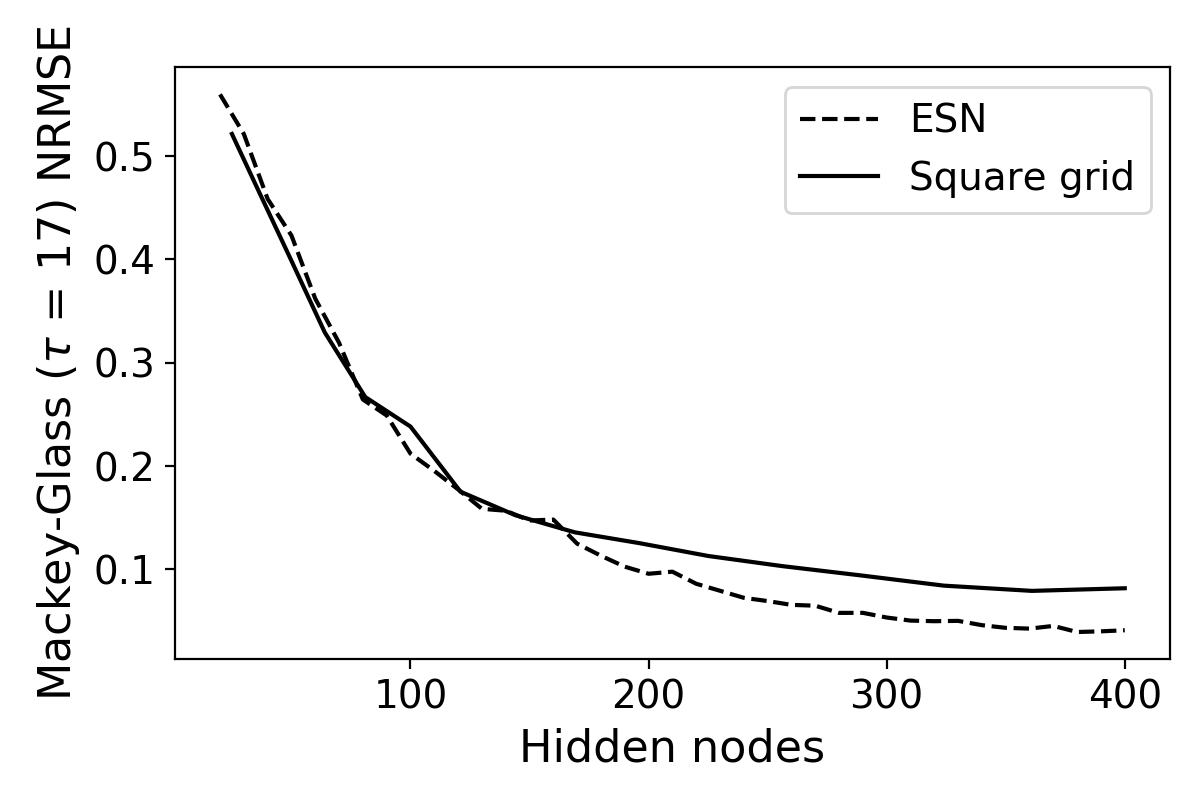
\includegraphics[width=3.5in]{figures/mg17.png}
  \caption{
    \textcolor{red}{
      No caption yet.
    }
  }
  \label{fig:mg17}
\end{figure}

\section{Shrinking and Growing Square Grids}

\subsection{Synopsis}

\subsection{Results and Discussion}

\textcolor{blue}{
  ``Reservoir computing: Reducing network size and improving
predictionstability'', as well as another paper in mailbox is about simplifying
networks (other is about Shanon information). Maybe useful to talk discuss these
as introduction.
}

\begin{figure}
  \centering
  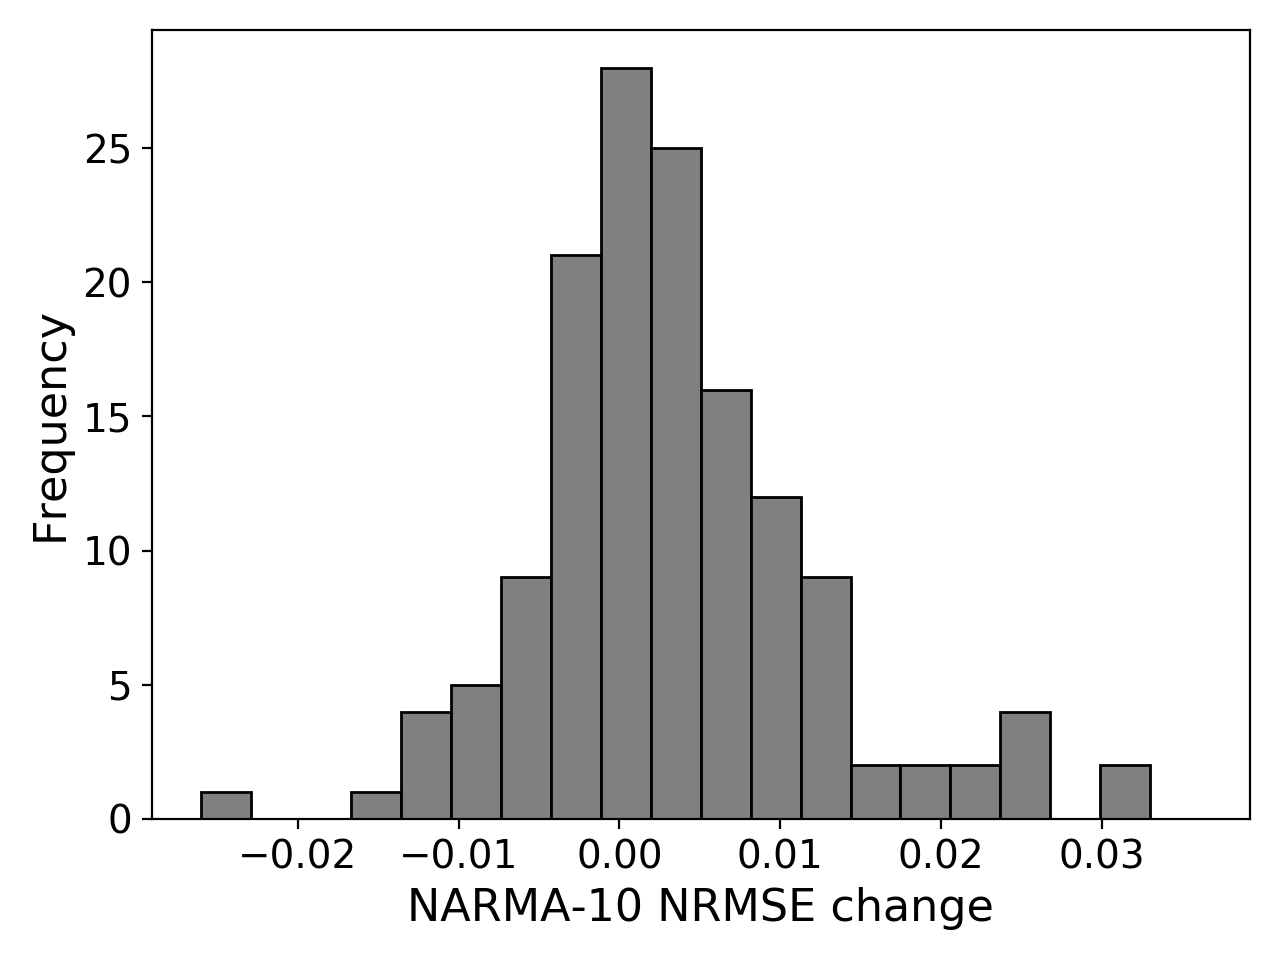
\includegraphics[width=3.5in]{figures/removal-hist.png}
  \caption{
    \textcolor{red}{
      Impact on NARMA-10 NRMSE when removing nodes from a 12x12 square grid
reservoir. No nodes are absolutely essential, while some removals actually
improve overall performance.
    }
  }
  \label{fig:rt-removal-hist}
\end{figure}

\begin{figure}
  \centering
  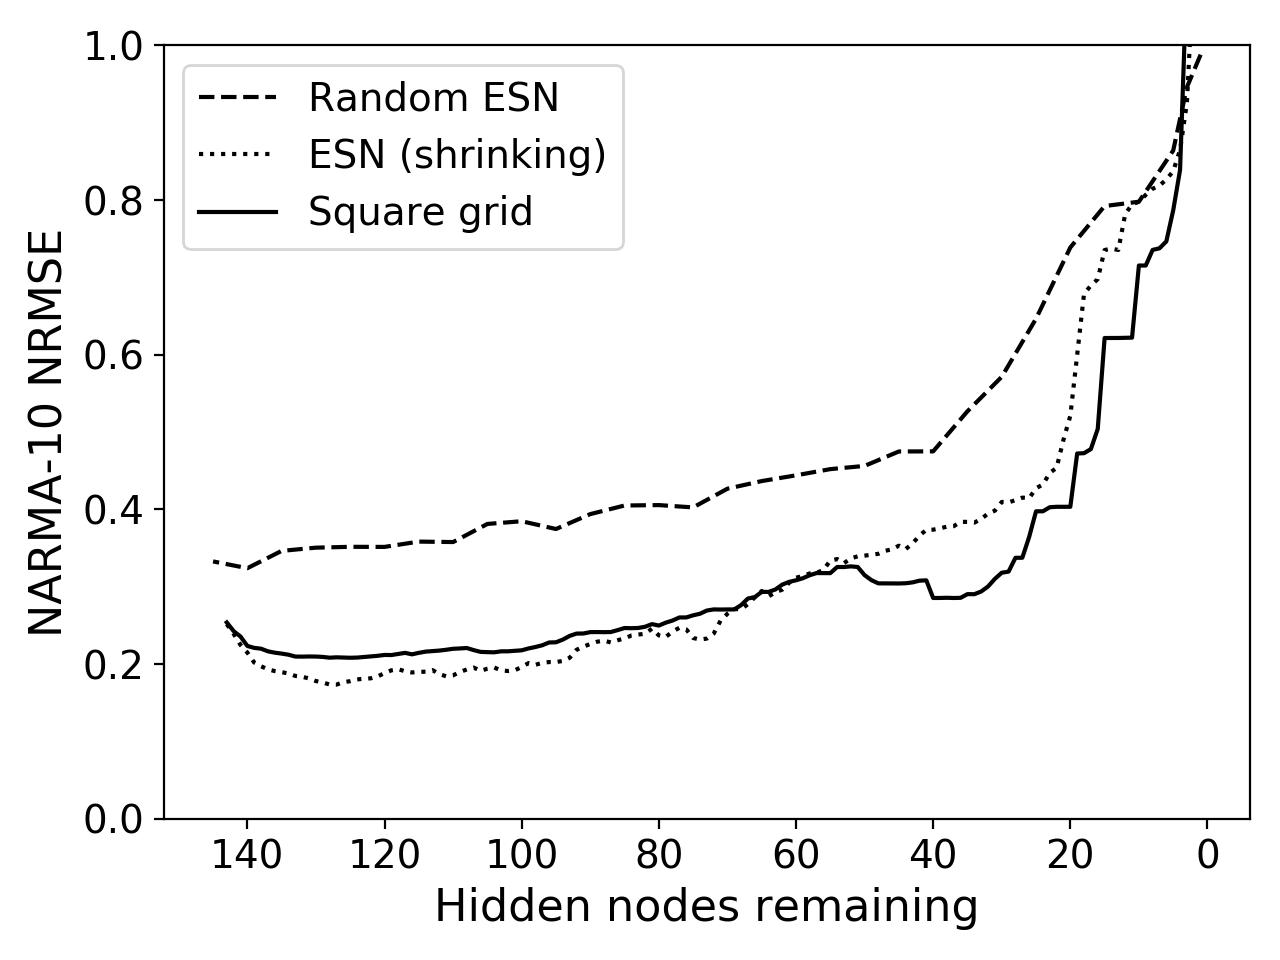
\includegraphics[width=3.5in]{figures/shrink-performance.png}
  \caption{
    \textcolor{red}{
      No caption yet.
    }
  }
  \label{fig:sq-shrink-performance}
\end{figure}

% (TODO): t!
\begin{figure*}[t]
  \centering
  \begin{subfigure}{.40\textwidth}
    \centering
    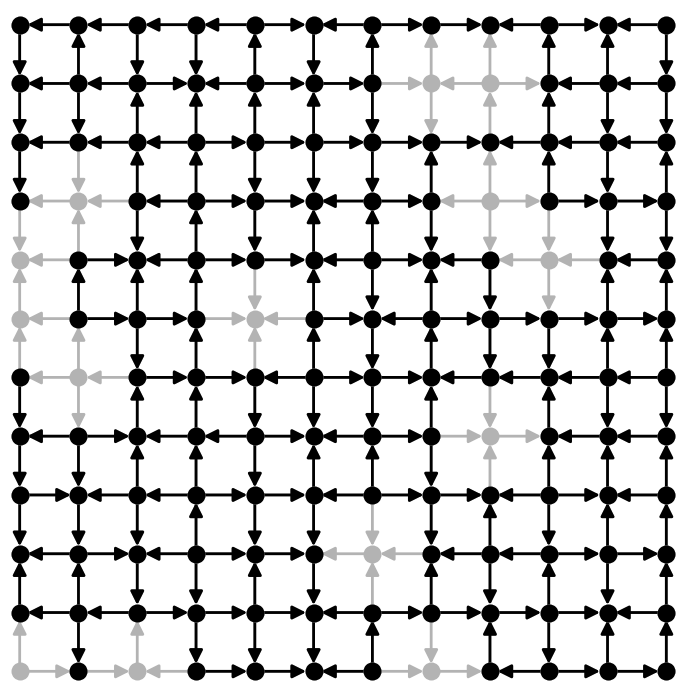
\includegraphics[width=1.0\linewidth]{figures/sq-grid-130.png}
    \caption{}
    \label{fig:sq-grid-130}
  \end{subfigure}
  \begin{subfigure}{.40\textwidth}
    \centering
    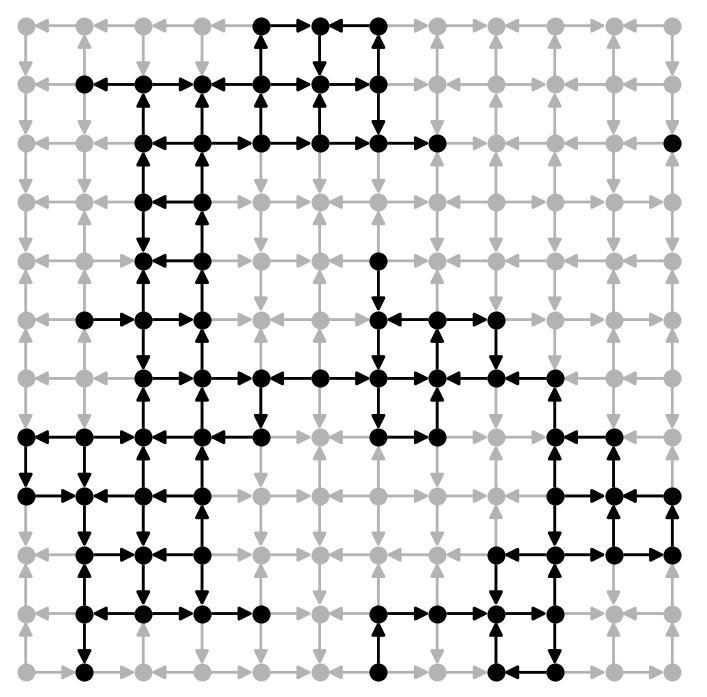
\includegraphics[width=1.0\linewidth]{figures/sq-grid-70.png}
    \caption{}
    \label{fig:sq-grid-70}
  \end{subfigure}
  \vskip\baselineskip

  \begin{subfigure}{.40\textwidth}
    \centering
    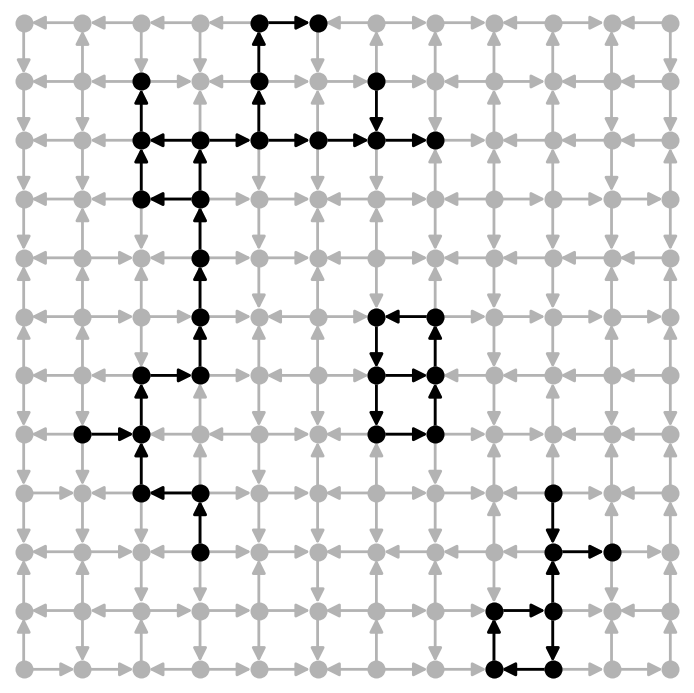
\includegraphics[width=1.0\linewidth]{figures/sq-grid-35.png}
    \caption{}
    \label{fig:sq-grid-35}
  \end{subfigure}
  \begin{subfigure}{.40\textwidth}
    \centering
    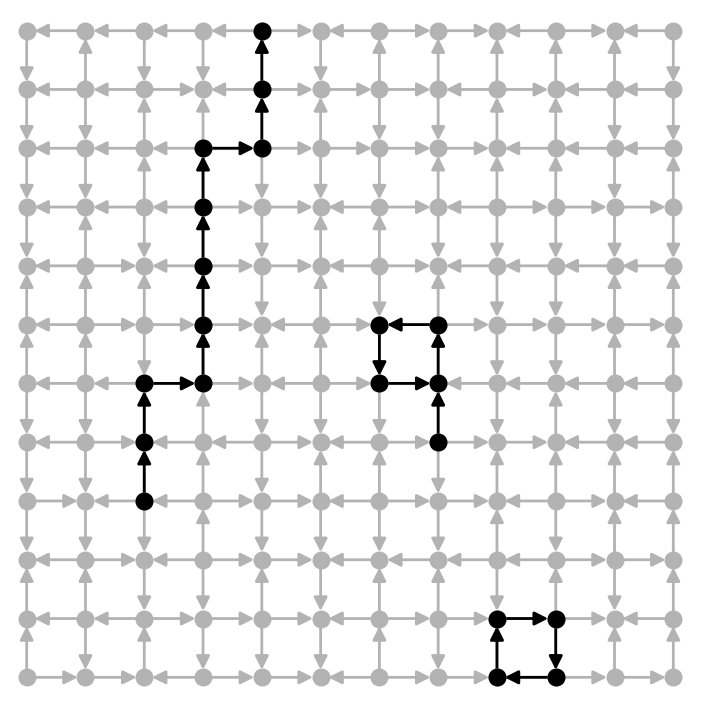
\includegraphics[width=1.0\linewidth]{figures/sq-grid-20.png}
    \caption{\textcolor{red}{Should have NRMSE and nodes left here.}}
    \label{fig:sq-grid-20}
  \end{subfigure}
  \caption{
    \textcolor{red}{
      Progression when incrementally removing nodes from a 12x12 square grid.
    }
  }
  \label{fig:sq-grid}
\end{figure*}

\textcolor{red}{
  Add the example when we have removed nodes from ESN? The one that is just
impossible to make sense of. This is common knowledge however, we could probably
just mention that.
}

\textcolor{red}{
  We need to stress that this is just one example, there is no variance here,
which is a bit of a weakness in the argument.
}

\begin{figure}
  \centering
  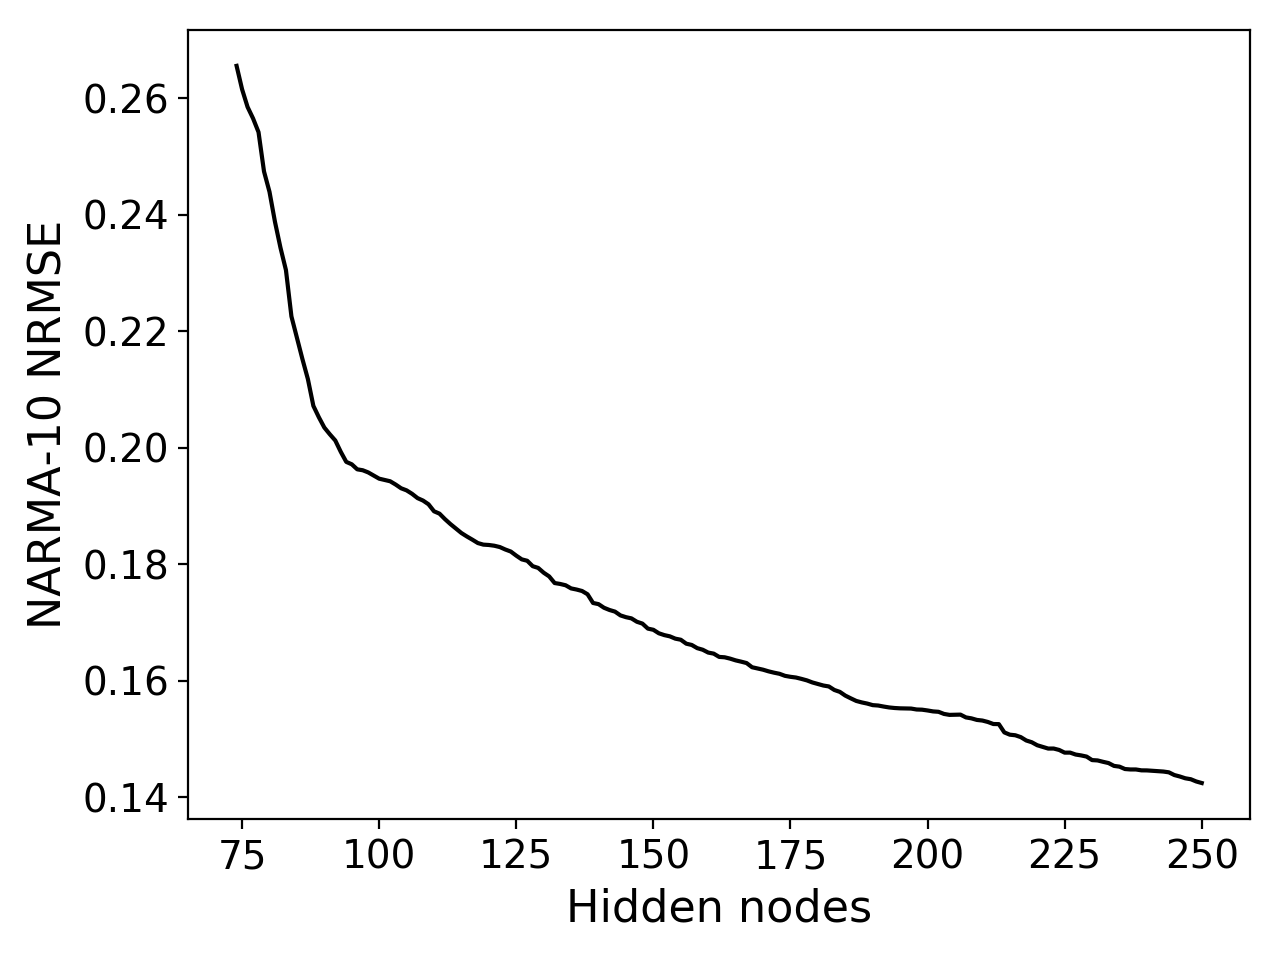
\includegraphics[width=3.5in]{figures/grow-performance.png}
  \caption{
    \textcolor{red}{
      No caption yet.
    }
  }
  \label{fig:sq-grow-performance}
\end{figure}

% (TODO): t!
\begin{figure*}[t]
  \centering
  \begin{subfigure}{1.0\textwidth}
    \centering
    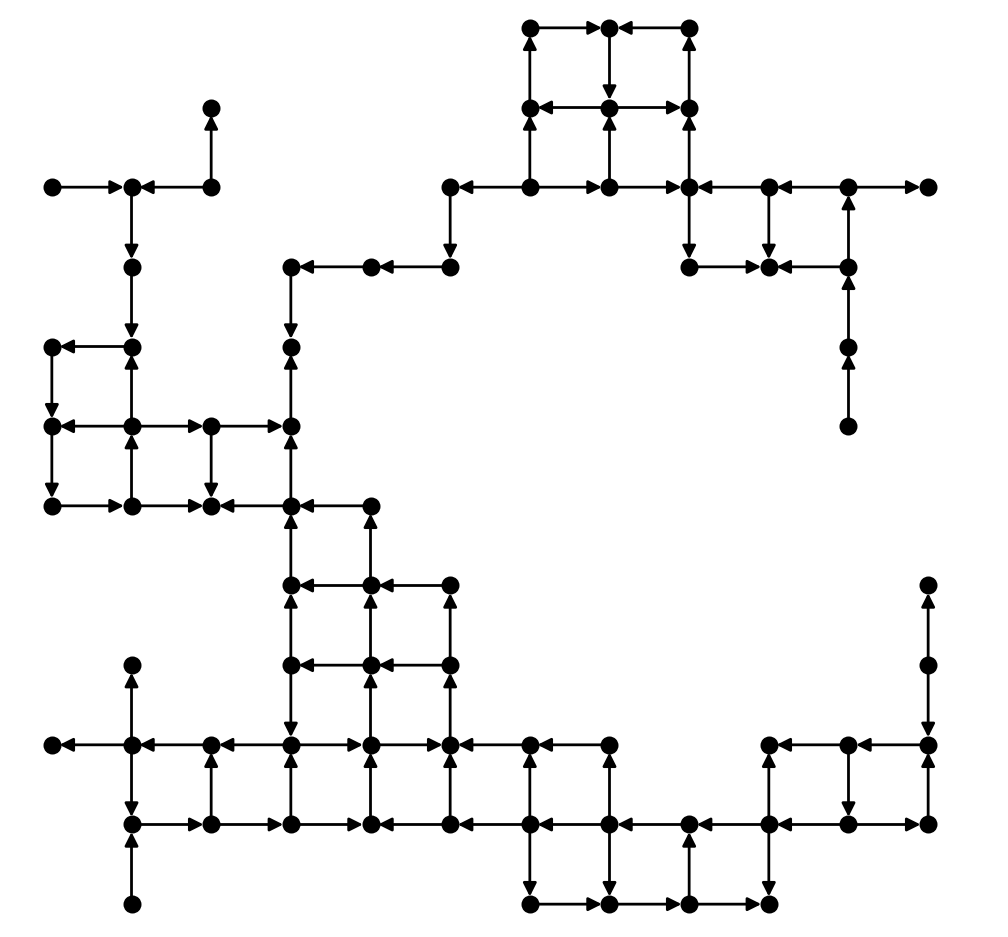
\includegraphics[width=0.5\linewidth]{figures/sq-grid-grow-74.png}
    \caption{}
    \label{fig:sq-grid-grow-74}
  \end{subfigure}
  \begin{subfigure}{.49\textwidth}
    \centering
    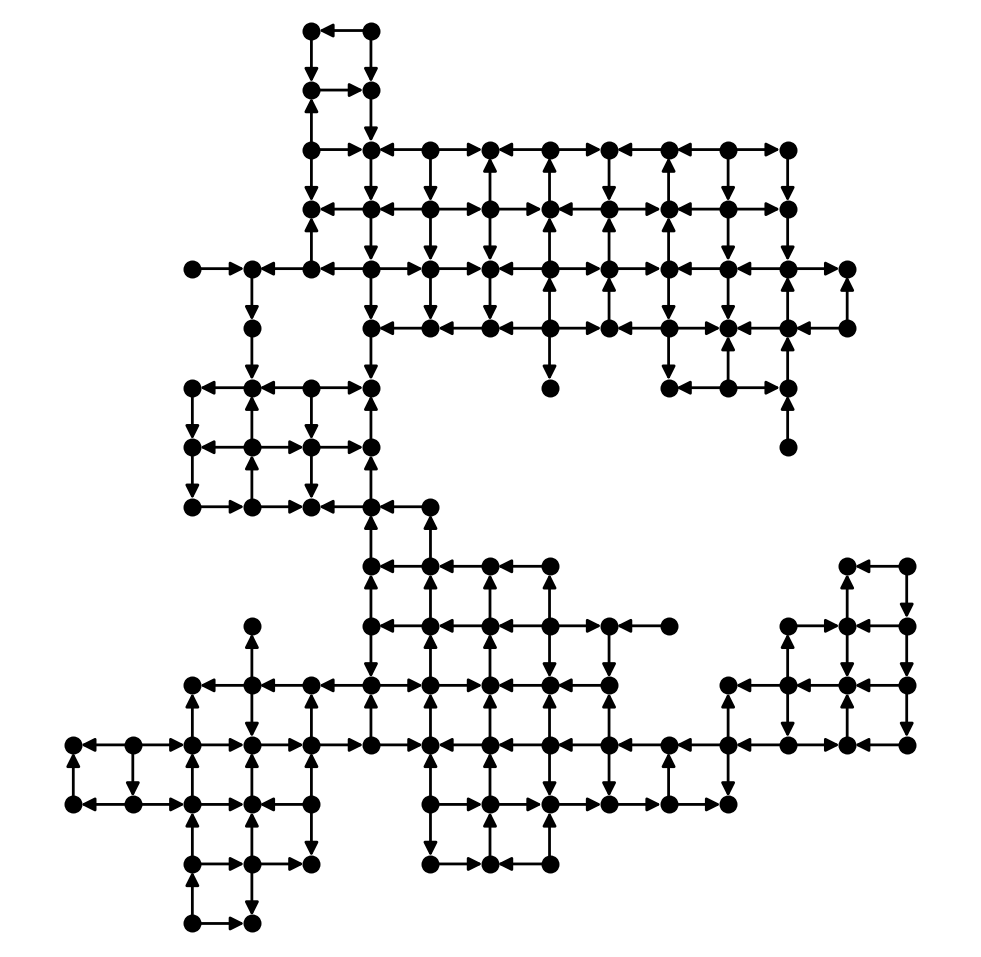
\includegraphics[width=1.0\linewidth]{figures/sq-grid-grow-124.png}
    \caption{}
    \label{fig:sq-grid-grow-124}
  \end{subfigure}
  \begin{subfigure}{.49\textwidth}
    \centering
    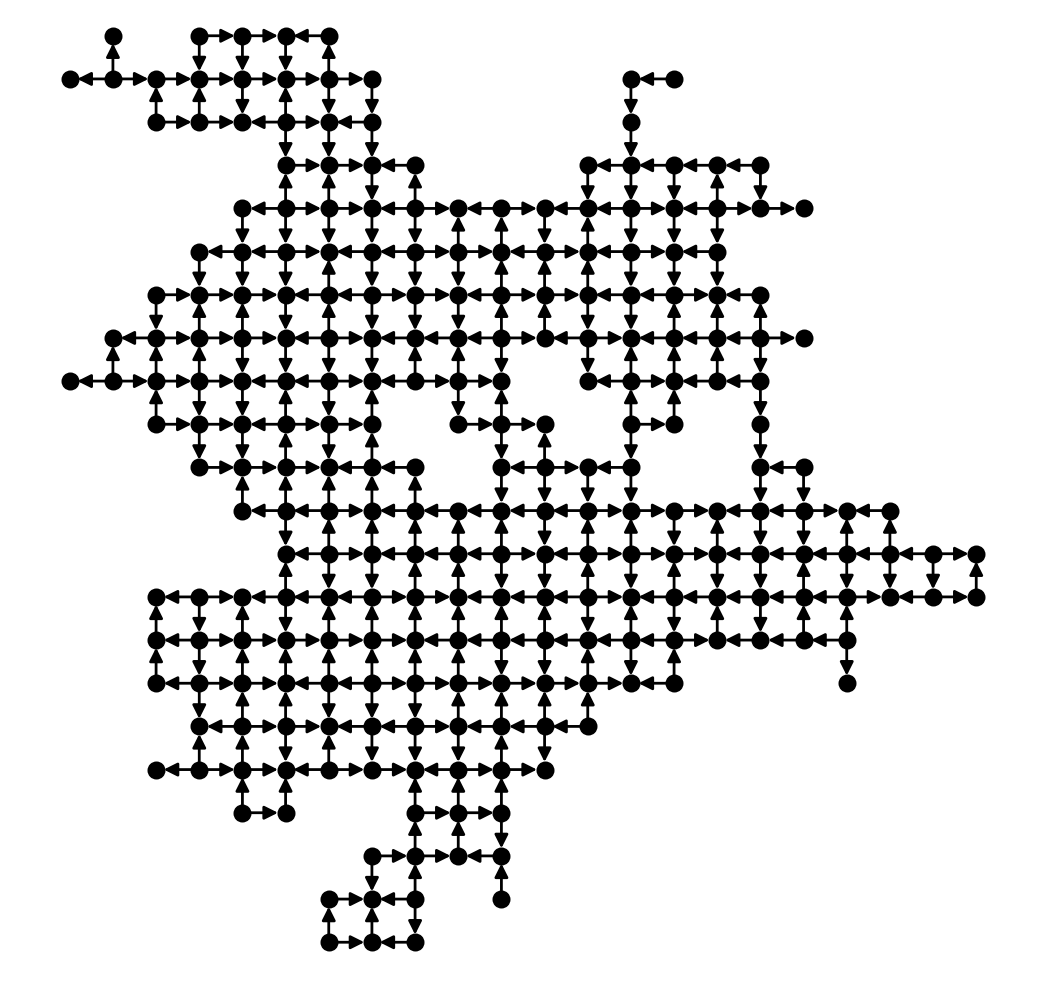
\includegraphics[width=1.0\linewidth]{figures/sq-grid-grow-250.png}
    \caption{\textcolor{red}{Should have captions for NRMSE and size.}}
    \label{fig:sq-grid-grow-250}
  \end{subfigure}
  \caption{
    \textcolor{red}{
      Caption. We see the initial reservoir from where we start growing in (a),
and progress in (b, c).
    }
  }
  \label{fig:sq-grid-grow}
\end{figure*}

\textcolor{red}{
  We repeat the experiment, but this time \textit{adding} nodes along the
frontier, as we can exhaust every possibility for every iteration without that
much trouble. Harder to see what is happening now.
}

\section{Restoring Bidirectional Edges}

\subsection{Synopsis}

\subsection{Results and Discussion}

\begin{figure}
  \centering
  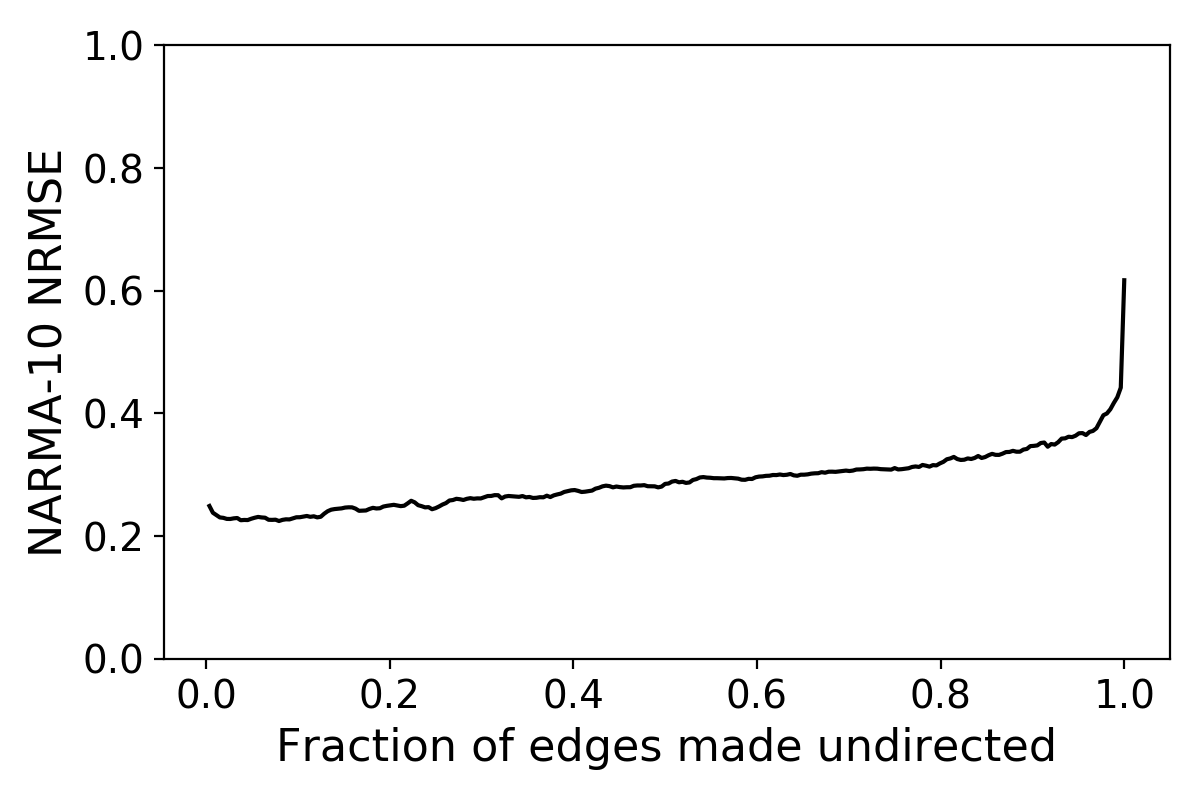
\includegraphics[width=3.5in]{figures/undir-performance.png}
  \caption{
    \textcolor{red}{
      No caption yet. 12x12 square grid.
    }
  }
  \label{fig:undirection-performance}
\end{figure}

\textcolor{red}{
  Imagine something similar to that of Figure \ref{fig:dir-lattice}, where now
only a fraction of the edges are directed again. However, we cannot directly
compare this to that of a cross section of that plot, as we have changed our
input scheme to be global, instead of the uniform distribution that was used
before.
}

\section{Conclusions}

\textcolor{red}{
  Remember that we are not necessarily concerned with finding really good square
grids, but rather that they work at all, since we are concerned with spatial
constraints.
}

\textcolor{red}{
  We find square grids to slightly outperform ESNs on NARMA, and about as good
on MG17.
}

\textcolor{red}{
  We find directedness to be important, and \textit{sufficient}. We find a type
of ESN that is fairly deterministic like CRJ, but has some freedom in
structure. This is useful for exploring ESNs.
}

\textcolor{red}{
  We underline a discrepancy between KQ and actual performance that is already
seen with CRJ. This is quite interesting.
}

\textcolor{red}{
  By analyzing removal of nodes, we find that there seems to be a ``core'' stem
for solving the NARMA task. And ``augmenting'' nodes around. This might be
telling about what happens in ESNs also, but due to randomness.
}

\textcolor{red}{
  We find that removing nodes and evaluating can be good to remove noisy nodes.
}


%%% Local Variables:
%%% mode: latex
%%% TeX-master: "../thesis"
%%% End:
